\documentclass[10pt]{examdesign}
\usepackage{amsmath}
\usepackage{enumitem}
\usepackage{amsfonts}
\usepackage{pgfplots}
\usepackage{pifont}
\usepackage{graphicx}
\usepackage{fancyhdr}
\usepackage{cancel}
\usepackage{gensymb}
\SectionFont{\large\sffamily}
\Fullpages
\ContinuousNumbering


\DefineAnswerWrapper{}{}
\NumberOfVersions{2}
%\IncludeFromFile{foobar.tex}
\examname{Quiz:  Angular Kinematics}
\class{ {\Large Physics}}

\def \namedata {Name: \hrulefill\\ 
	Date: \hrulefill \\
	Period: \hrulefill \\
	Peer Reviewer: \hrulefill \\
	Authentication Code: \hrulefill
	\\
	
	\begin{tabular}{| p{1cm} | p{1cm} | p{1 cm} | p{1cm} |}
		\hline
		+1 & 0 & -1 & $\Sigma$ 
		\\
		\hline
		& & & \vspace{.5cm}
		\\ \hline
		
	\end{tabular}
	\\
	\vspace{-.6in}
	
}




\begin{document}




\begin{multiplechoice} [title={Multiple Choice},
	rearrange=yes]
	\textit{Choose the best answer to each question.}
	\begin{question}
		Angular \word{{velocity}{acceleration}} is represented by the variable - 
		\choice {$\theta$}
		\choice {\word{{$\alpha$}{$\omega$}}}
		\choice [!]{\word{{$\omega$}{$\alpha$}}}
		\choice {$\Delta$}
	\end{question}

	\begin{question}
	 	What is the angular equivalent of the linear equation $ v_f = v_i + a t$?
		\choice {$\omega_{avg} = \frac{\omega_i + \omega_f}{2}$}
		\choice [!]{$\omega_f = \omega_i + at$}
		\choice {$\theta = \omega_i t + \frac{1}{2}\alpha t^2$}
		\choice {$\omega_f^2 = \omega_i^2 + 2 \alpha \theta $ }
	\end{question}

	\begin{question}
		A rotating wheel has a constant angular acceleration.  It has an initial angular velocity of 4 rad/s, and 5 seconds later has a final angular velocity of 9 rad/s.  What is the object's angular displacement?
		\choice {1 rad}
		\choice {2.5 rad}
		\choice [!]{32.5 rad}
		\choice {138.888 rad}
	\end{question}



	\begin{question}
	An object has an angular acceleration of $13 rad/s^2$.  What is its angular velocity after 7 seconds?
		\choice{13 rad/s}
		\choice{45.5 rad/s}
		\choice{91 rad/s}
		\choice[!]{It cannot be determined.}
	\end{question}
	
	\begin{question}
	How many radians is 1/4 of a rotation?
		\choice{90 rad}
		\choice[!]{$\frac{\pi}{2}$ rad}
		\choice{$\frac{\pi}{4}$ rad}
		\choice{$2 \pi$ rad}
	\end{question}
	
	\begin{question}
		Which of the following best describes how the speed of an object's rotation is changing?
		\choice{Angular Displacement}
		\choice{Angular Velocity}
		\choice{Angular Acceleration}
		\choice{None of the above}
	\end{question}

	\begin{question}
	Which of the following are the angular kinematic variables?
		\choice{$\theta$, $\omega$, $\alpha$, $\Delta$, and $t$.}
		\choice{$\theta_i$, $\theta_f$, $\omega$, $\alpha$, and $t$.}
		\choice{$\theta$, $\omega_i$, $\omega_f$, $\alpha$, and $t$.}
		\choice[!]{$\theta$, $\omega$, $\alpha_i$, $\alpha_f$, and $t$.}
	\end{question}

\begin{question}
	A soda can has a radius of 0.02 m.  If it rolls 12 times, what is the distance the can will roll? 
	\choice[!]{1.26 m}
	\choice{1.108 m}
	\choice{.72m}
	\choice{.36 m}
\end{question}





\begin{block}

		\textbf{The following two questions refer to the following information:} 
		The picture below shows an overhead view of China's Z-20 Anti-submarine helicopter.  Two points have been labeled A and B.  
		
				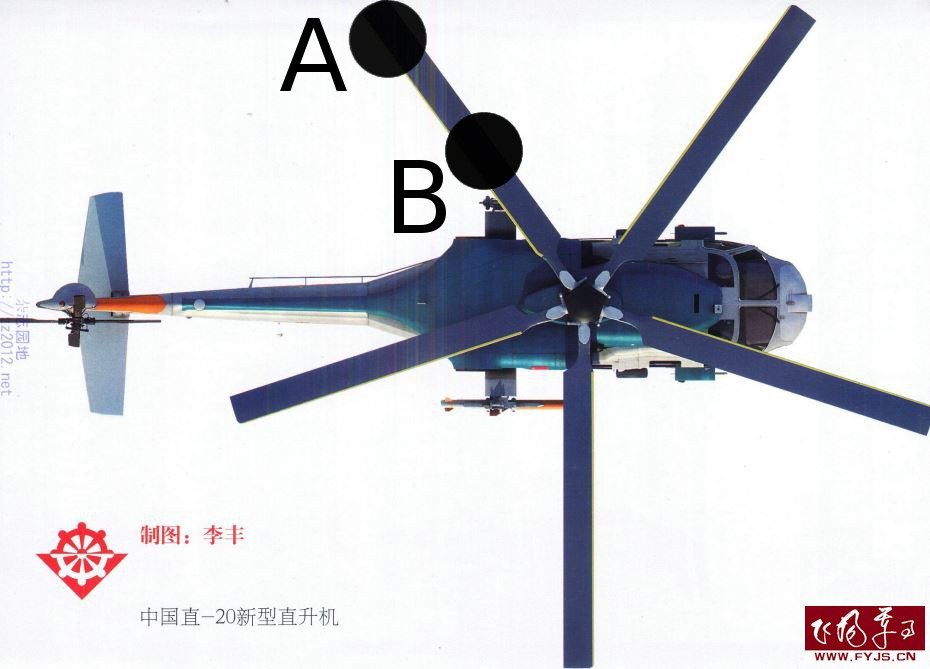
\includegraphics[height=3cm]{heli.jpg}
	

	
\begin{question}
When the helicopter blades are rotating, which point has a greater \underline{angular velocity ($\omega$)}?
	
	\vspace{0.1in}

		\choice{A}
		\choice{B}
		\choice[!]{They both have the same angular velocity}
		\choice{It is impossible to tell.}
\end{question}

\begin{question}
	When the helicopter blades are rotating, which point has a greater \underline{linear velocity (v)}?
	
	\vspace{0.1in}
	
	\choice{A}
	\choice{B}
	\choice[!]{They both have the same angular velocity}
	\choice{It is impossible to tell.}
\end{question}



\end{block}
	\end{multiplechoice}




\end{document}
